\chapter{Fundamentação teórica}

\section{PISCINAS e sua manutenção}

    \subsection{HISTÓRICO E POPULARIZAÇÃO DAS PISCINAS}
    
        O termo piscina, que vem do latim piscis (“peixe”), pode ser definido como um tanque cheio de água destinado a diversos fins, sejam eles natação, mergulho, saltos ornamentais ou simplesmente recreação\cite{piscinaOquee}. Há registros de piscinas desde 2600 a.C., como “Os Grandes Banhos de Mohenjodaro”, considerado um dos primeiros tanques públicos de água, construído em tijolos e revestido com gesso. Contudo, acredita-se que esse tanque tenha sido feito apenas para fins religiosos.
         \begin{figure}[H]
         	\centering
         	\caption{ }  
        	\centering
         	\label{fig:cont}
        	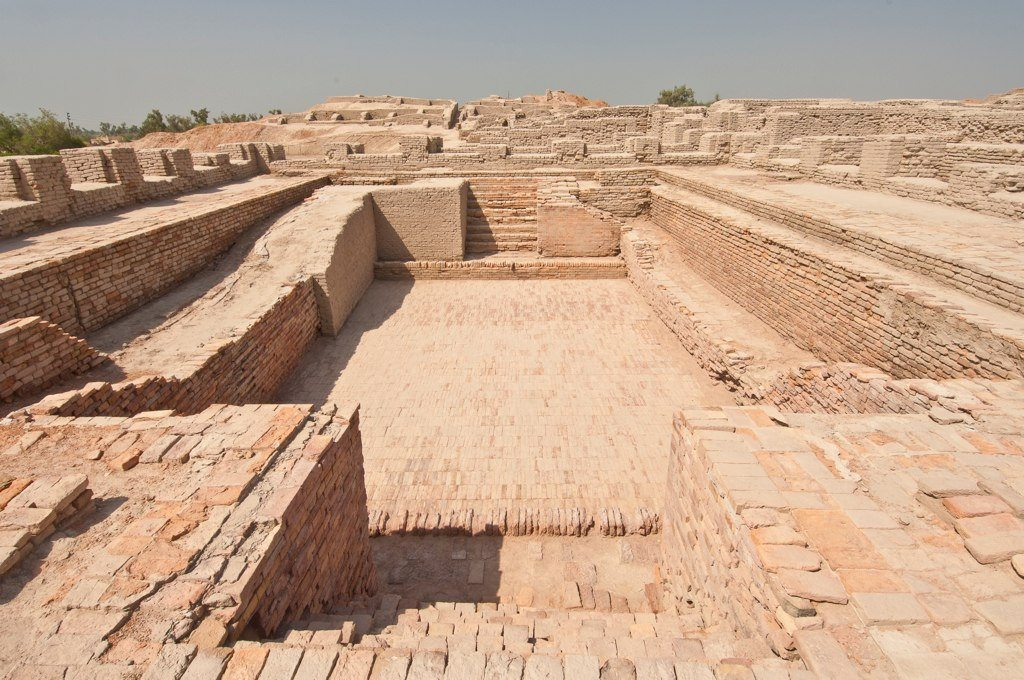
\includegraphics[width=0.78\textwidth]{imagens/primeiraPiscina.png}
        	\caption*{Fonte: Fibratec}
         \end{figure}
        
        Com o avanço da tecnologia no século XX, as piscinas passaram a incorporar novos sistemas, como os de cloração e filtração, que permitiram manter a água limpa sem a necessidade de trocas completas, prática que antes era essencial. No Ocidente, as piscinas começaram a se popularizar com a invenção do gunite (mistura de cimento, areia e água), um material que facilitava a instalação, possibilitava projetos mais flexíveis e reduzia consideravelmente o custo de construção\cite{piscinaHistoria}.

    \subsection{COMPONENTES BÁSICOS DE UMA PISCINA}
        
        \textcolor{black}{Segundo \cite{refComponents}, as piscinas, de forma abstrata, são estruturas extremamente simples, consistindo basicamente em grandes reservatórios de água destinados ao uso recreativo. Podem existir diferentes tipos, como piscinas de ondas de parques aquáticos, particulares, públicas, entre outras. Contudo, em sua maioria, todas as piscinas possuem alguns componentes básicos necessários para o processo de filtração e tratamento químico.}

        \textcolor{black}{Diante disso, é importante ter uma noção mínima dos componentes que compõem uma piscina. São eles: bomba motorizada, filtro de água, alimentador químico, drenos, devoluções e encanamentos de PVC\footnote{Sigla para Poli(cloreto de vinila), um polímero termoplástico versátil, conhecido por sua durabilidade, resistência química e ampla utilização em tubos, conexões e revestimentos.}. Em alguns casos, pode haver também um aquecedor, com o objetivo de manter a temperatura da água em níveis mais elevados.}

        \begin{itemize}
        
            \item \textcolor{black}{Bomba Motorizada:}
                \textcolor{black}{Responsável por circular toda a água, puxando-a da bacia e conduzindo-a até os demais processos.}

            \item \textcolor{black}{Filtro de Água:}
                \textcolor{black}{Remove parte das impurezas da água, como folhas, poeira e micro-organismos.}

            \item \textcolor{black}{Alimentador Químico:}
                \textcolor{black}{Distribui os produtos químicos responsáveis pela limpeza e manutenção da qualidade da água.}

            \item \textcolor{black}{Drenos:}
                \textcolor{black}{Removem a água utilizada em processos de limpeza, escoamento ou manutenção.}

            \item \textcolor{black}{Devoluções:}
                \textcolor{black}{Pontos de reabastecimento da água na piscina.}

            \item \textcolor{black}{Encanamentos de PVC:}
                \textcolor{black}{Interligam todos os componentes da piscina, permitindo o transporte adequado da água.}
                %Colocar uma imagem de cada item respectivo ou uma no final que tenha todos
                
        \end{itemize}

        \begin{figure}[H]
         	\centering
         	\caption{ }  
        	\centering
         	\label{fig:cont}
        	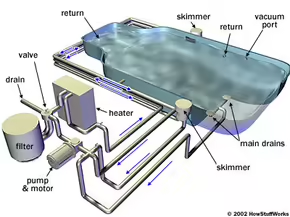
\includegraphics[width=0.48\textwidth]{imagens/componentesPiscina.png}
            \caption*{Componentes básicos de uma piscina}
        	\caption*{Fonte: \cite{refComponents}}
         \end{figure}

        \textcolor{black}{Todos esses componentes têm como objetivo bombear a água em um ciclo contínuo, fazendo-a passar por todos os sistemas, como filtragem e tratamento químico. Além disso, existem também componentes responsáveis por auxiliar na limpeza física da piscina, que serão abordados a seguir.}

        \subsubsection*{Aspirador de escova}

         \textcolor{black}{Segundo \cite{benedito2024projeto}, o aspirador de escova é um dos itens mais importantes na limpeza física da piscina, tendo como função a aspiração da sujeira acumulada no fundo.}

            \begin{figure}[H]
                \centering
                \caption{ }  
                \centering
                \label{fig:cont}
                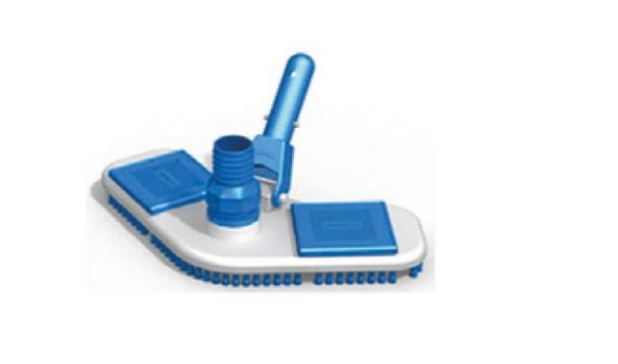
\includegraphics[width=0.60\textwidth]{imagens/aspirador.png}
                \caption*{Aspirador de escova}
                \caption*{Fonte: \cite{benedito2024projeto}}
            \end{figure}

        \subsubsection*{Peneira}

         \textcolor{black}{A peneira é responsável pela coleta de resíduos, como insetos, plásticos e pequenas folhas que ficam flutuando na superfície da piscina \cite{benedito2024projeto}.}

            \begin{figure}[H]
                \centering
                \caption{ }  
                \centering
                \label{fig:cont}
                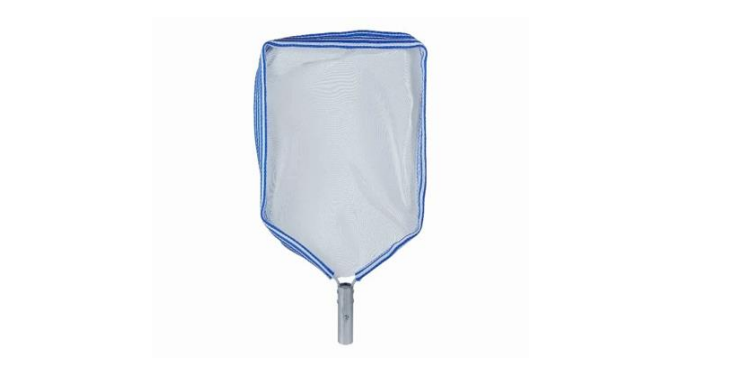
\includegraphics[width=0.60\textwidth]{imagens/peneira.png}
                \caption*{Peneira}
                \caption*{Fonte: \cite{benedito2024projeto}}
            \end{figure}

        \subsubsection*{Escova}

         \textcolor{black}{De acordo com o \cite{benedito2024projeto}, a escova é um dos principais equipamentos utilizados na limpeza da piscina. É responsável pela remoção de poeira e algas das paredes, podendo também ser utilizada na limpeza do fundo.}

            \begin{figure}[H]
                \centering
                \caption{ }  
                \centering
                \label{fig:cont}
                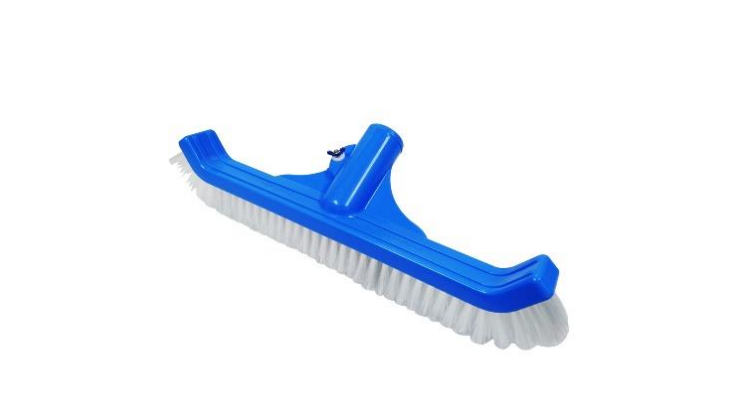
\includegraphics[width=0.60\textwidth]{imagens/escova.png}
                \caption*{Escova}
                \caption*{Fonte: \cite{benedito2024projeto}}
            \end{figure}

        \subsubsection*{Cabo de alumínio}

         \textcolor{black}{O cabo de alumínio tem a função de se encaixar nos equipamentos citados anteriormente. Está disponível em diversos tamanhos, garantindo melhor conforto e praticidade no momento do manuseio \cite{benedito2024projeto}.}

            \begin{figure}[H]
                \centering
                \caption{ }  
                \centering
                \label{fig:cont}
                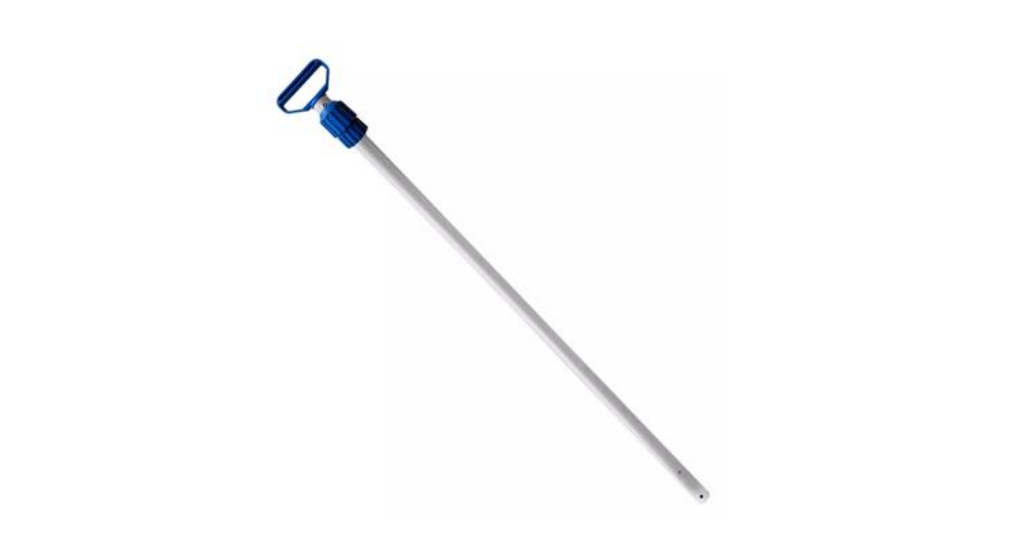
\includegraphics[width=0.60\textwidth]{imagens/cabo}.png
                \caption*{Cabo de alumínio}
                \caption*{Fonte: \cite{benedito2024projeto}}
            \end{figure}

        Portanto, é entendível que a manutenção de uma piscina envolve diversos componentes essenciais para uma limpeza eficiente. Cada componente possui um papel fundamental para garantir a circulação, filtração e tratamento adequados da água. 
        
        Esses elementos, aliados a boas práticas de operação e manutenção, formam a base para o funcionamento eficiente do sistema. Contudo, a eficiência desse processo não depende apenas dos equipamentos mecânicos, mas também dos procedimentos técnicos e químicos que asseguram a qualidade da água. 
        
        Sendo assim, o próximo tópico abordará as normas e os procedimentos técnicos de limpeza manual, indispensáveis para a preservação da saúde do usuário.
        

    \subsection{NORMAS E PROCEDIMENTOS TÉCNICOS DE LIMPEZA MANUAL}

       \textcolor{black}{Segundo \cite{piscineiroProfissional}, a falta de um procedimento correto de limpeza pode acarretar sérios problemas de saúde para os usuários da piscina, como dermatite, micose e outras infecções. O tratamento deve ser constante e realizado de forma eficiente, de modo que os resultados estejam sempre em conformidade com as normas estabelecidas pela Associação Brasileira de Normas Técnicas ABNT\footnote{Associação Brasileira de Normas Técnicas, responsável por estabelecer as diretrizes de padronização para trabalhos acadêmicos no Brasil.}. De acordo com \cite{guiaTratamento}, existem diversos fatores poluentes presentes em uma piscina, como suor e urina, pelos e cabelos, óleos da pele, insetos, folhas, formação de algas, entre outros.}

       \textcolor{black}{Esses poluentes podem afetar diretamente os parâmetros químicos da piscina, como o pH e o nível de cloro. Segundo o mesmo autor, ao realizar apenas a limpeza física, utilizando escovas ou redes, é possível remover somente a parte visível dos resíduos, como folhas, insetos e lodo. Por essa razão, torna-se necessária a aplicação de um tratamento químico eficaz, uma vez que poluentes como suor e urina se misturam à água, e os sistemas de filtragem são incapazes de removê-los completamente.}

       %Tentar inserir alguma imagem no final de algum desses três paragrafos pois esta tudo muito grande

       \textcolor{black}{É de suma importância que a água de uma piscina limpa atenda a determinados pré-requisitos, tais como: ausência de bactérias do grupo coliforme ou Staphylococcus aureus\footnote{Bactéria coco Gram-positiva, frequentemente encontrada na pele e nas fossas nasais humanas, responsável por infecções de gravidade variável.}, boa visibilidade do fundo, superfície livre de sujeiras e pH dentro da faixa ideal, entre 7,2 e 7,8.}

       Para que esses parâmetros sejam alcançados, é essencial que a água apresente três princípios básicos:
    
       \begin{itemize}
            \item \textbf{\textcolor{black}{Água Limpa:}} \textcolor{black}{Água transparente e sem a presença de sedimentos.}
            
            \item \textbf{\textcolor{black}{Água Balanceada:}} \textcolor{black}{Segundo todos os parâmetros prescritos, sem risco de prejudicar o banhista.}
             
            \item \textbf{\textcolor{black}{Água Saudável:}} \textcolor{black}{Livre de micro-organismos que podem vir a prejudicar o banhista.}
            
        \end{itemize}

        \begin{figure}[H]
                \centering
                \caption{ }  
            	\centering
                \label{fig:cont}
            	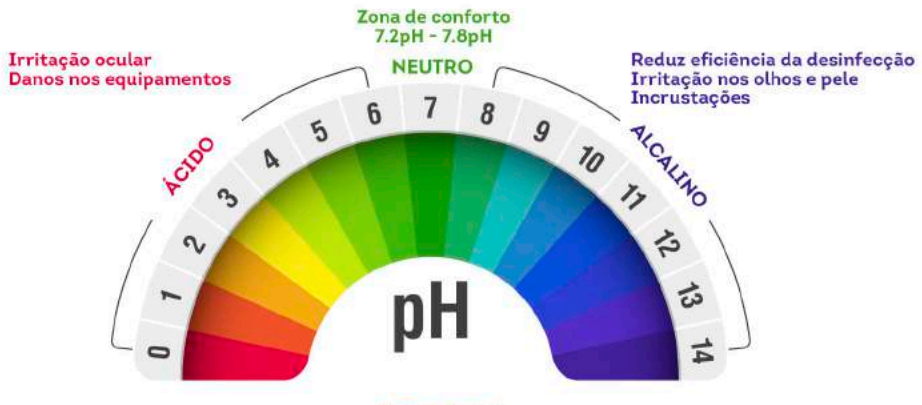
\includegraphics[width=0.48\textwidth]{imagens/medidorPh.png}
                \caption*{Faixa de pH}
            	\caption*{Fonte: \cite{guiaTratamento}}
        \end{figure}


        \textcolor{black}{Antes do processo de limpeza, é fundamental conhecer a área e o volume da piscina, para que seja utilizada a quantidade correta de produtos e se obtenha uma higienização eficiente, sem desperdícios.}

        O cálculo da área e do volume pode variar de acordo com o formato da piscina, sendo possível aplicar diferentes fórmulas geométricas para cada caso.

        \subsubsection*{\textcolor{black}{Piscina Retangular}}
        
            \[
            A = \text{comprimento} \times \text{largura}
            \]
            \[
            V = \text{comprimento} \times \text{largura} \times \text{profundidade}
            \]
            
        \subsubsection*{\textcolor{black}{Piscina Circular}}
            \[
            A = \pi r^2
            \]
            \[
            V = \pi r^2 h
            \]
            
        \subsubsection*{\textcolor{black}{Piscina Oval (Elíptica)}}
            \[
            A = \pi \cdot \frac{a}{2} \cdot \frac{b}{2}
            \]
            \[
            V = A \cdot h
            \]
            
            \textcolor{black}{Nos casos em que a piscina possui fundo inclinado, a profundidade considerada deve ser a média entre a parte mais rasa e a mais funda:}
            \[
            h_m = \frac{h_{\text{maior}} + h_{\text{menor}}}{2}
            \]
            

        \textcolor{black}{Segundo \cite{tccSilva}, o processo de limpeza é semelhante ao utilizado em indústrias, como nas estações de tratamento de água, seguindo uma sequência de cinco etapas:}

        \begin{itemize}
            \item \textbf{\textcolor{black}{Oxidação:}} \textcolor{black}{ocorre a mistura do cloro com o objetivo de oxidar metais como ferro e manganês, facilitando a remoção de matéria orgânica.}
            
            \item \textbf{\textcolor{black}{Coagulação e Floculação:}} \textcolor{black}{consiste na adição de sulfato de alumínio e, ocasionalmente, cloreto férrico, para promover o desequilíbrio das partículas, seguido da circulação da água, o que possibilita a formação de flocos.}
             
            \item \textbf{\textcolor{black}{Decantação:}} \textcolor{black}{acontece quando as partículas coaguladas e floculadas se depositam no fundo da piscina devido à circulação lenta do fluido. Dependendo do produto utilizado, essa etapa pode durar cerca de seis horas.}

            \item \textbf{\textcolor{black}{Filtração:}} \textcolor{black}{etapa responsável pela retenção do acúmulo de sujeira proveniente das etapas anteriores, geralmente realizada por meio de um filtro de areia.}

            \item \textbf{\textcolor{black}{Correção de pH:}} \textcolor{black}{consiste na análise e no ajuste do pH da água, normalmente com o uso de um medidor para identificar o valor. Esse procedimento é essencial para evitar a deterioração das tubulações e equipamentos.}
            
        \end{itemize}

        \textcolor{black}{Em virtude do exposto, torna-se evidente que a aplicação correta dos procedimentos técnicos estabelecidos é indispensável para a manutenção da qualidade da água. Nesse sentido, a precisão e a segurança demandadas pelo processo dependem diretamente da escolha e do manuseio adequado dos produtos químicos, tema que será abordado na próxima seção.}


    \subsection{PRODUTOS QUÍMICOS E ACESSÓRIOS USADOS NA LIMPEZA DE PISCINAS}

        \textcolor{black}{O tratamento correto e bem executado durante a limpeza de uma piscina, tanto físico quanto químico, é essencial para garantir a qualidade da água, evitando possíveis infecções ou doenças de origem hídrica. Por isso, é fundamental compreender quais produtos utilizar, como utilizá-los e qual a melhor forma de realizar o tratamento físico.}

        O principal objetivo desta seção é apresentar os produtos e ferramentas recomendados para assegurar a qualidade da água e preservar a saúde dos usuários.

        \begin{itemize}
        
            \item \textbf{\textcolor{black}{Precedimento Químico:}} \textcolor{black}{Segundo \cite{guiaTratamento}, o procedimento químico envolve todas as etapas relacionadas à adição de substâncias químicas à água, com o intuito de garantir sua qualidade e prevenir riscos à saúde dos banhistas. Esses produtos ajustam a alcalinidade, o pH e realizam a desinfecção da água, eliminando micro-organismos e bactérias por meio do uso de cloro e outros compostos destinados ao controle dos parâmetros químicos.}

                \begin{figure}[H]
                    \centering
                    \caption{ }  
                	\centering
                    \label{fig:cont}
                	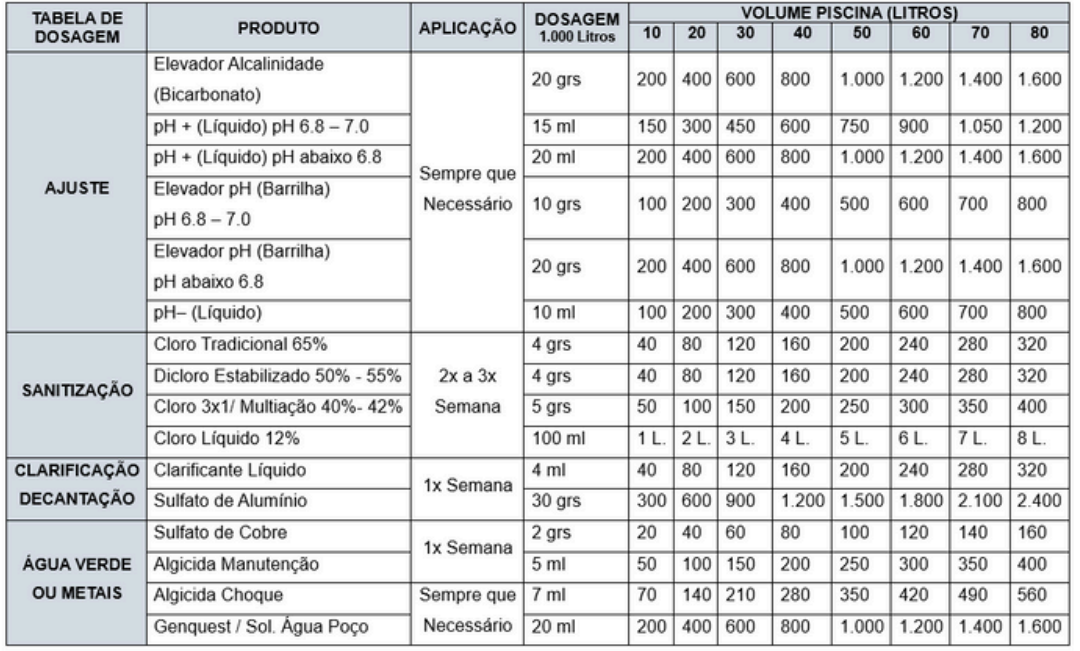
\includegraphics[width=1.00\textwidth]{imagens/tabelaProdutos.png}
                    \caption*{Tabela de Dosagem de Produtos}
                	\caption*{Fonte: \cite{guiaTratamento}}
                \end{figure}
    
                \begin{itemize}
    
                    \item \textbf{\textcolor{black}{Elevador de Alcalinidade:}} \textcolor{black}{a alcalinidade da água está relacionada à sua capacidade de neutralizar ácidos, funcionando como uma barreira para manter o pH estável. O produto tem como função elevar a alcalinidade para o nível ideal, entre 80 e 120 ppm.}
    
                    \item \textbf{\textcolor{black}{Barrilha, Elevador de pH, pH+:}} \textcolor{black}{produtos de composição alcalina utilizados para elevar o pH quando ele está abaixo do ideal.}
    
                    \item \textbf{\textcolor{black}{Redutor de pH, pH-:}} \textcolor{black}{produtos de composição ácida que têm a função de diminuir o pH da água.}
    
                    \item \textbf{\textcolor{black}{Hipoclorito de Sódio, Cloro, Dicloro, Multiação 3x1:}} \textcolor{black}{agentes sanitizantes que têm como objetivo eliminar micro-organismos presentes na água}
    
                    \item \textbf{\textcolor{black}{Sulfato de Alumínio, Clarificantes:}} \textcolor{black}{provocam o processo de decantação, em que as partículas de sujeira são aglomeradas e levadas ao fundo da piscina, facilitando as etapas de aspiração e filtração.}
    
                    \item \textbf{\textcolor{black}{Sulfato de Cobre, Algicida:}} \textcolor{black}{utilizados quando a piscina apresenta coloração esverdeada, auxiliando na eliminação de algas e lodo.}
    
                    \item \textbf{\textcolor{black}{Genquest, Solução Água de poço:}} \textcolor{black}{empregados para remover manchas e colorações provocadas por metais dissolvidos na água.}
    
                \end{itemize}
                
            \item \textbf{\textcolor{black}{Medição de Parâmetros e Ajuste do pH:}} \textcolor{black}{Para medir os parâmetros da água, utilizam-se estojos de análise específicos para cada variável a ser verificada. O ajuste correto desses parâmetros é essencial para um tratamento eficiente e seguro.}

            \begin{figure}[H]
                    \centering
                    \caption{ }  
                	\centering
                    \label{fig:cont}
                	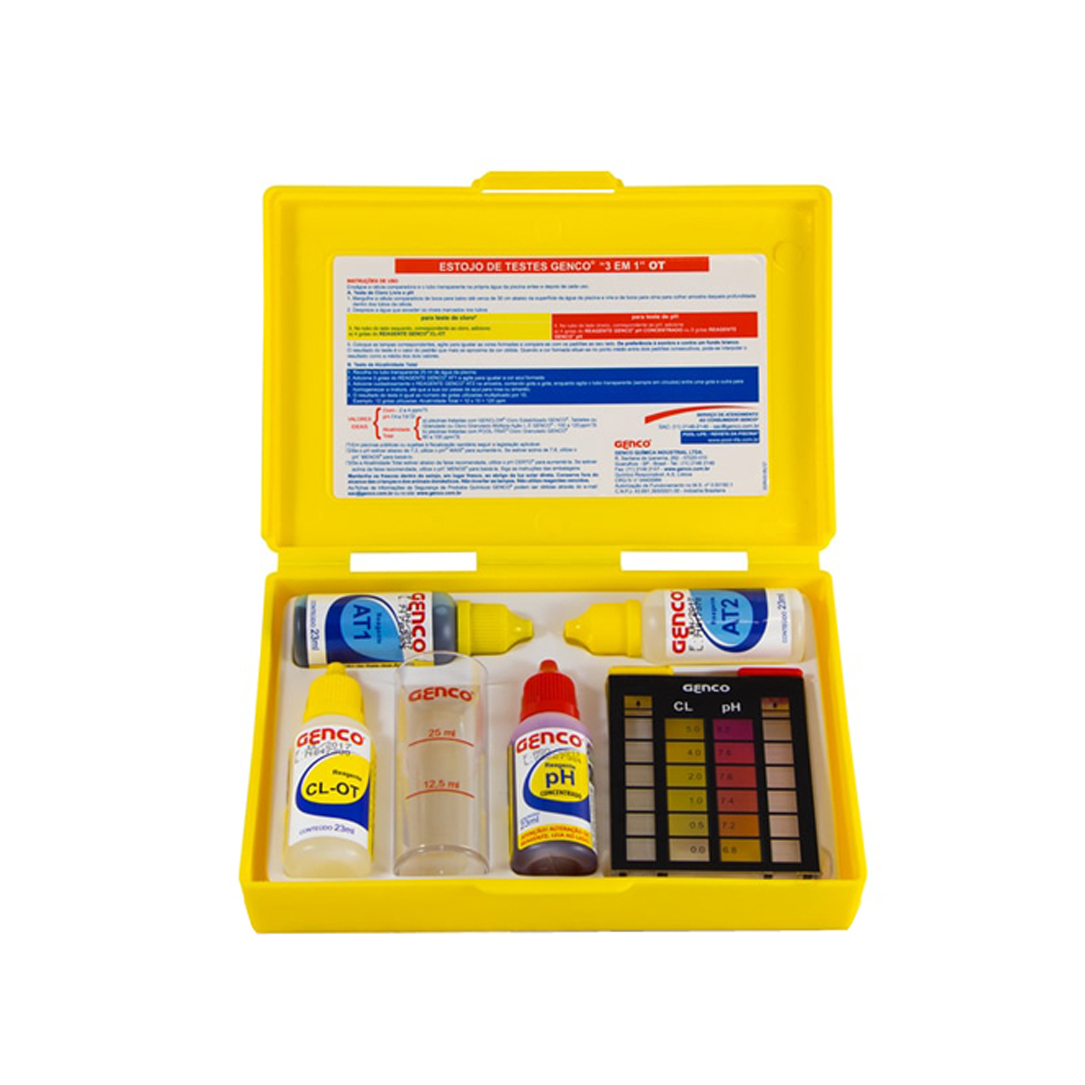
\includegraphics[width=0.48\textwidth]{imagens/estojoMedidor.png}
                    \caption*{Estojo para Análise de Parâmetros}
                	\caption*{Fonte: \cite{gencoEmpresa}}
            \end{figure}

            %Colocar imagens de medidor
            \textcolor{black}{Os produtos a serem aplicados dependem dos resultados obtidos nas análises químicas. Caso o pH esteja abaixo de 7,0, deve-se utilizar o elevador de pH ou barrilha. Se a alcalinidade estiver inferior ao valor ideal, aplica-se o elevador de alcalinidade. Por fim, se o nível de cloro estiver baixo, é necessário adicionar cloro líquido ou granulado, conforme a tabela apresentada anteriormente.}


            \item \textbf{\textcolor{black}{Limpeza química:}} \textcolor{black}{Com base nas informações apresentadas, compreende-se que a turbidez da água, caracterizada pela presença de partículas em suspensão, é um dos principais indicadores da necessidade de tratamento químico. Para corrigir esse problema, recomenda-se o uso de um decantador, que aglomera as partículas e as leva ao fundo da piscina, permitindo sua posterior aspiração.}
            
            \begin{itemize}
                \item \textbf{\textcolor{black}{Clarificação:}} \textcolor{black}{utilizada quando a água está opaca e sem brilho; realiza-se com produtos clarificantes específicos.}
                
                \item \textbf{\textcolor{black}{Floculação ou decantação:}} \textcolor{black}{aplicadas quando a água se encontra turva ou suja; para isso, adiciona-se floculante líquido ou decantador em pó (geralmente, sulfato de alumínio).}
            \end{itemize}

            Após a aplicação dos produtos, recomenda-se aguardar entre 6 e 12 horas antes de iniciar o processo de aspiração do fundo da piscina.

            %\textcolor{red}{colocar imagens de piscinas verdes e opacas, no final de tudo ou após a citação de cada uma}
            
        \end{itemize}

        \textcolor{black}{Com todos os dados e informações apresentados, é possível compreender o processo necessário para realizar uma limpeza eficiente de piscina. Entretanto, esse procedimento pode se mostrar complexo para algumas pessoas, motivo pelo qual surgem alternativas tecnológicas, especialmente por meio da automação residencial, que será abordada na próxima seção.}
         
   
\section{FUNDAMENTOS DA AUTOMAÇÃO RESIDENCIAL}
    \textcolor{black}{A automação residencial é um conceito que se baseia no conjunto de serviços voltados para a satisfação de necessidades básicas com o uso da tecnologia em uma residência, como: segurança, comunicação, etc. Tais necessidades são atendidas por meio da integração de sistemas que permitem a realização de tarefas de forma programada, promovendo praticidade e eficiência.}

    \textcolor{black}{O que realmente define uma instalação residencial automatizada é a forma como os sistemas se integram, aliada à capacidade de executar tarefas mediante instruções programáveis. Essa integração deve abranger todos os sistemas da residência, como a instalação elétrica, segurança, multimídia, comunicação e utilidades \cite{automacaoResidencialCap1}.}

    \textcolor{black}{Um dos principais objetivos da automação residencial é porporcionar comodidade e segurança ininterrupta aos moradores, com o constante auxílio dos computadores e sistemas inteligentes. Alguns exemplos incluem satélites que controlam o trânsito e sistemas automatizados presente em residências \cite{algunsAspectos}. Além disso, existem outras denominações que se referem à automação residencial, como domótica, casas conectadas e casas inteligentes. O termo domótica tem origem no latim domus (“casa”), combinado com a palavra “robótica”, representando a união entre o lar e a tecnologia \cite{automacaoTecnologiaPraticidade}}

    \textcolor{black}{A automação residencial é composta por um conjunto de benefícios fundamentais que estruturam o conceito de casa inteligente. Entre seus principais pilares, destacam-se:}

    \begin{itemize}
        \item \textbf{\textcolor{black}{Conforto:}} \textcolor{black}{sendo um dos pilares centrais, tem como objetivo facilitar as tarefas cotidianas. A automação proporciona maior comodidade ao usuário, permitindo o controle remoto de lâmpadas, ar-condicionados, sistemas de irrigação, entre outros \cite{automacaoTecnologiaPraticidade}.}
        
        \item \textbf{\textcolor{black}{Segurança:}} \textcolor{black}{a integração de câmeras, fechaduras eletrônicas e sensores de luz e presença torna a segurança um dos principais benefícios da automação. Isso possibilita o monitoramento remoto da residência, reforçando os aspectos de proteção, praticidade e conforto \cite{automacaoTecnologiaPraticidade}.}
        
        \item \textbf{\textcolor{black}{Economia:}} \textcolor{black}{a automação também contribui para o uso racional de energia, por meio de sistemas que desligam lâmpadas automaticamente e ajustam a climatização conforme a necessidade. Dessa forma, evita-se o desperdício e promove-se maior eficiência energética \cite{automacaoTecnologiaPraticidade}.}
        
    \end{itemize}

    \textcolor{black}{Para que a automação funcione de forma adequada, é necessário o uso de dispositivos com conectividade, acesso à internet e um sistema central de controle capaz de realizar a coleta e troca de informações entre os equipamentos.}

    Praticamente todos os aparelhos eletrônicos que possuem algum tipo de acionamento podem ser automatizados, como sistemas de iluminação, portões, climatização e segurança. Esses dispositivos são conectados a uma central de controle, que pode ser acessada por meio de um display touch\footnote{O display touch é uma superfície sensível ao toque que permite a interação direta do usuário}, localizado na própria central, aplicativos para smartphones ou comandos de voz \cite{automacaoTecnologiaPraticidade}.

    \subsection{HISTÓRICO E EVOLUÇÃO DA AUTOMAÇÃO RESIDENCIAL}
        \textcolor{black}{é uma tecnologia relativamente recente no mercado, mas que se encontra em constante evolução. Por volta de 1970, nos Estados Unidos, surgiram os primeiros módulos inteligentes, cujos comandos eram transmitidos pela rede elétrica da residência por meio da tecnologia PLC\footnote{Controlador Lógico Programável. Consiste em um tipo de computador industrial para automação e controle de processos.}. Contudo, seu funcionamento era bastante simples, permitindo apenas ligar e desligar remotamente alguns equipamentos e sistemas de iluminação \cite{automacaoResidencialCap1}.}

        \textcolor{black}{De acordo com \cite{automacaoResidencialCap1}, o surgimento de tecnologias como os computadores pessoais e a internet impulsionou significativamente o avanço das soluções residenciais inteligentes, tornando-as mais aceitas e utilizadas. Em países com economias mais desenvolvidas, o conceito de casa inteligente apresentou grande crescimento e sofisticação nos últimos anos.}

        A seguir, apresenta-se uma tabela que ilustra a evolução de algumas das principais tecnologias utilizadas na automação residencial:

        \begin{table}[H]
            \centering
            \renewcommand{\arraystretch}{1.3}
            \setlength{\tabcolsep}{10pt}
            \begin{tabular}{lccccc}
            \hline
            \textbf{Tecnologia} & \textbf{2003} & \textbf{2004} & \textbf{2005} & \textbf{2006} & \textbf{2015(*)} \\
            \hline
            Cabeamento estruturado & 42\% & 61\% & 49\% & 53\% & 80\% \\
            Monitoramento de segurança & 18\% & 28\% & 29\% & 32\% & 81\% \\
            Multiroom audio & 9\% & 12\% & 15\% & 16\% & 86\% \\
            Home Theater & 9\% & 8\% & 11\% & 12\% & 86\% \\
            Controle de iluminação & 1\% & 2\% & 6\% & 8\% & 75\% \\
            Automação integrada & 0\% & 2\% & 6\% & 6\% & 70\% \\
            Gerenciamento de energia & 1\% & 5\% & 11\% & 11\% & 62\% \\
            \hline
            \end{tabular}
            \caption{Evolução das tecnologias de automação residencial ao longo dos anos.}
            \label{tab:tecnologias-automacao}

            \vspace{0.5em}
            \small
            \textbf{Fonte:} \cite{automacaoResidencialCap1}.\\
        \end{table}

        \textcolor{black}{Dessa forma, ao compreender a evolução histórica e o crescimento das tecnologias aplicadas à automação residencial, torna-se evidente a importância de conhecer os fundamentos técnicos que sustentam esse campo.}

        No próximo tópico, serão abordados alguns dos principais conceitos e componentes que compõem a base dos sistemas automatizados, como controladores, sensores, atuadores e protocolos de comunicação. Esses elementos são essenciais para o entendimento do funcionamento e da integração entre os dispositivos que possibilitam a automação em ambientes residenciais.


    \subsection{CONCEITOS TÉCNICOS DE AUTOMAÇÃO RESIDENCIAL}
    
       \textcolor{black}{Tecnicamente denominada domótica, a automação residencial tem como principal objetivo acionar, monitorar, integrar e controlar diferentes tipos de variáveis ou cargas de uma residência, como iluminação, climatização, áudio e vídeo, com o intuito de gerar eficiência, comodidade e segurança para o usuário \cite{oliveira2019domotica}.}

       No Brasil, o termo mais comumente utilizado é automação residencial, traduzido diretamente da expressão americana \textit{home automation}. Contudo, essa tradução não abrange totalmente o significado do termo domótica. O uso de novas tecnologias no país vem crescendo exponencialmente; entretanto, o mercado da construção civil ainda não acompanha o mesmo ritmo de evolução tecnológica observado em setores como o automotivo, que já utiliza amplamente tecnologias embarcadas\footnote{Computador especializado, composto por hardware e software, que executa uma função dedicada dentro de um sistema maior} \cite{hipolito2018automaccao}.

       \textcolor{black}{De acordo com \cite{accardi2012automaccao}, a forma como os componentes se comunicam está diretamente relacionada à arquitetura adotada, que pode ser centralizada ou descentralizada.}

       Em uma arquitetura centralizada, todos os componentes do sistema respondem a um único dispositivo, que por sua vez, deve ter uma alta inteligência e desempenho.

        \begin{figure}[H]
                \centering
                \caption{ }  
                \centering
                \label{fig:cont}
                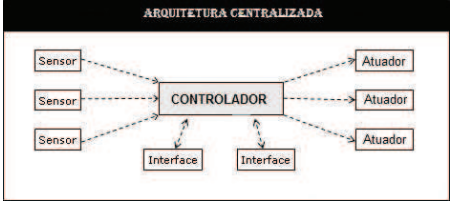
\includegraphics[width=0.53\textwidth]{imagens/arquiteturaCentralizada.png}
                \caption*{Arquitetura centralizada}
                \caption*{Fonte: \cite{hipolito2018automaccao}}
        \end{figure}

       \textcolor{black}{Já na arquitetura descentralizada, diversos controladores coexistem e se comunicam entre si por meio de um barramento de dados\footnote{Refere-se a um sistema onde a comunicação e a coordenação entre os componentes são distribuídas, sem depender de uma autoridade ou ponto central}, compartilhando o controle dos dispositivos conectados.}

        \begin{figure}[H]
                \centering
                \caption{ }  
                \centering
                \label{fig:cont}
                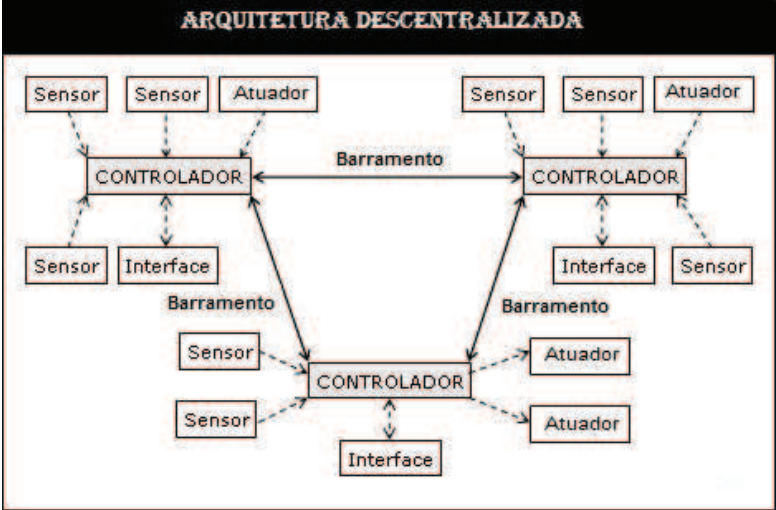
\includegraphics[width=0.53\textwidth]{imagens/arquiteturaDescentralizada.png}
                \caption*{Arquitetura descentralizada}
                \caption*{Fonte: \cite{hipolito2018automaccao}}
         \end{figure}

       \textcolor{black}{Para que toda a integração dos sistemas ocorra de forma eficiente, é necessário compreender alguns conceitos técnicos fundamentais, que possibilitam a execução bem-sucedida das funções automatizadas.}

       Nas seções seguintes, serão apresentados esses conceitos e componentes, essenciais para o entendimento do funcionamento da automação residencial.

       \subsubsection{COMPONENTES BÁSICOS}

        \textcolor{black}{A automação residencial tem seu funcionamento composto por diversos componentes, que variam desde sensores simples até centrais complexas de automação. A seguir, são apresentados alguns dos principais elementos que compõem essa estrutura:}

            \begin{itemize}
                \item \textbf{\textcolor{black}{Camadas de dispositivos:}} \textcolor{black}{(1)~Sensores: Segundo \cite{hipolito2018automaccao}, um sensor pode ser definido como um dispositivo sensível ao ambiente no qual está inserido, capaz de detectar alterações em variáveis como temperatura, luminosidade ou movimento. (2)~Atuadores: são componentes eletromecânicos acionados pelo sistema para executar uma função específica, como ativar uma sirene, lâmpada, fechadura magnética, motor ou válvula. (3)~Controladores: têm como função monitorar os parâmetros coletados pelos sensores e, de acordo com os dados obtidos, acionar o respectivo atuador vinculado. Podem possuir interfaces próprias ou fazer parte de grandes centrais de controle. (4)~Interfaces: dispositivos que permitem ao usuário interagir com o sistema automatizado, como aplicativos móveis, painéis digitais ou páginas web \cite{accardi2012automaccao}.}
                
                \item \textbf{\textcolor{black}{Camada de comunicação/rede:}} \textcolor{black}{Segundo \cite{accardi2012automaccao}, a camada de comunicação, também chamada de protocolo, “é um acordo entre as partes que se comunicam, estabelecendo como se dará a comunicação”. Assim, entende-se que um protocolo é, em resumo, o conjunto de regras e padrões utilizados para que diferentes dispositivos possam se comunicar entre si.}
                
                Entre os principais protocolos empregados na automação residencial, destacam-se: Ethernet, X-10, HomePNA e Wi-Fi. Alguns desses protocolos foram desenvolvidos especificamente para a automação residencial, enquanto outros foram adaptados de aplicações industriais e comerciais.
                
                \item \textbf{\textcolor{black}{Camada de controle/automação lógica:}} \textcolor{black}{A camada de controle, também chamada de central de automação, pode ser considerada o “cérebro” do sistema, sendo responsável por gerenciar todos os dispositivos conectados. Ela processa as informações de entrada e saída e executa as ações necessárias conforme as instruções programadas.}
                
                A configuração da central pode ser realizada por meio de um software dedicado, acessado através de um computador ou dispositivo móvel. Essa central é escalável\footnote{Descreve algo que pode crescer ou ser aumentado em magnitude, seja física ou figurativamente}, permitindo que novos dispositivos sejam adicionados ao sistema de forma contínua, conforme a necessidade de expansão.
        
            \end{itemize}
    

    \textcolor{black}{Diante de todos os dados e fundamentos apresentados, fica evidente que a automação residencial encontra-se em constante evolução, impulsionada pela integração de sensores, controladores, motores e protocolos de comunicação. Esses elementos, quando aplicados corretamente, possibilitam o desenvolvimento de sistemas inteligentes, capazes de automatizar e otimizar tarefas rotineiras.}

    Nesse contexto, o próximo capítulo abordará o desenvolvimento de um sistema automatizado de limpeza de piscinas, aplicando na prática os conceitos estudados e demonstrando como a integração entre hardware e software pode oferecer uma solução segura, eficiente e inovadora para a manutenção de piscinas residenciais.